\chapter{Appendix}

Turn over for the appendices.

\clearpage

\section{Appendix A - Gantt Charts}

\begin{center}
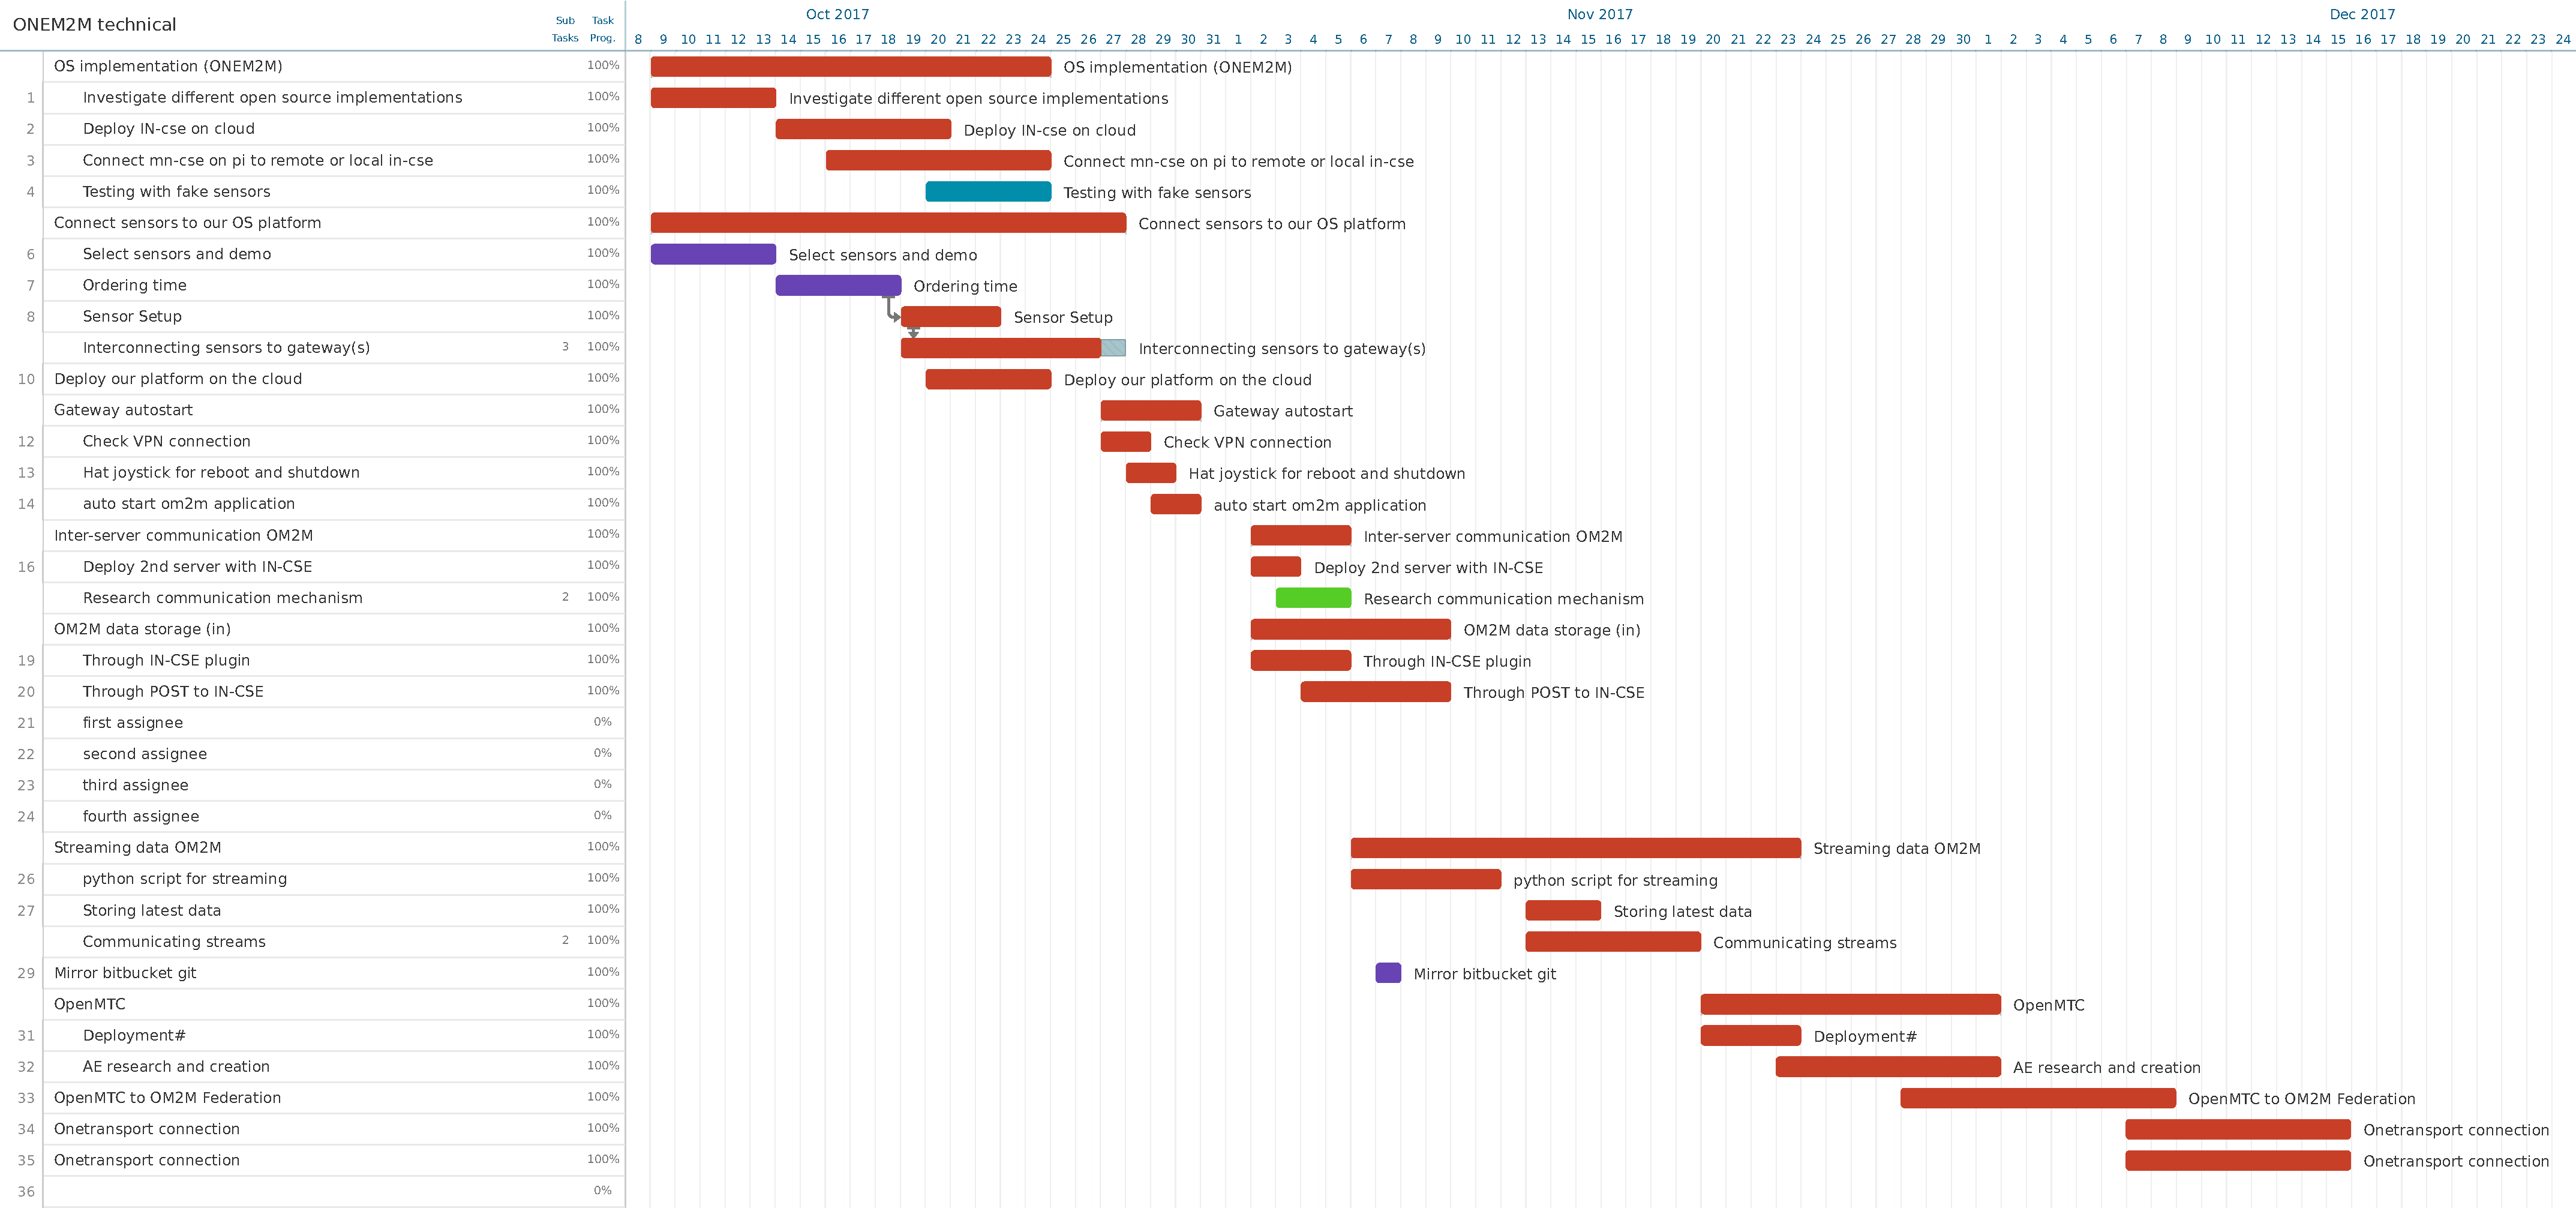
\includegraphics[scale=0.31,angle=90]{gatt}
\end{center}

\section{Appendix B - Communications Log}

The group met with the client, InterDigital on a weekly basis. Due to the clients London location, most were conducted over Skype, however a few were face to face. Additionally, the client was kept in the development loop with frequent emails asking for design input and implementation feedback. The list of email conversations can be found below:

\subsection*{OneTRANSPORT Federation Confirmation}
\label{sec:fed-conf}

\begin{lstlisting}
Great.
 
I was able to retrieve the contents of your CSE from a version of our CSE running locally:
 
+ curl -s -H 'Accept: application/json' -H 'X-M2M-RI: discover-remotecse2' -H 'X-M2M-Origin: CsuperAE' 'http://localhost:9011/~/in-cse-id/main?fu=1'
{
  "m2m:uril": [
    "/in-cse-id/main",
    "/in-cse-id/main/acp_admin",
    "/in-cse-id/main/mn-pi",
    "/in-cse-id/main/mn-pi/accelerometer_DATA",
    "/in-cse-id/main/mn-pi/camera_DATA",
    "/in-cse-id/main/mn-pi/camera_DATA/cin_145974492",
    "/in-cse-id/main/mn-pi/camera_DATA/cin_148737069",
    "/in-cse-id/main/mn-pi/camera_DATA/cin_183274186",
    "/in-cse-id/main/mn-pi/camera_DATA/cin_267279449",
    "/in-cse-id/main/mn-pi/camera_DATA/cin_307899785",
    "/in-cse-id/main/mn-pi/camera_DATA/cin_831851713",
    "/in-cse-id/main/mn-pi/camera_DATA/cin_865024078",
    "/in-cse-id/main/mn-pi/camera_DATA/cin_909142608",
    "/in-cse-id/main/mn-pi/camera_DATA/cin_928272334",
    "/in-cse-id/main/mn-pi/camera_DATA/cin_985322460",
    "/in-cse-id/main/mn-pi/compass_DATA",
    "/in-cse-id/main/mn-pi/cpu_DATA",
    "/in-cse-id/main/mn-pi/disk_DATA",
    "/in-cse-id/main/mn-pi/gyroscope_DATA",
    "/in-cse-id/main/mn-pi/humidity_DATA",
    "/in-cse-id/main/mn-pi/memory_DATA",
    "/in-cse-id/main/mn-pi/null_DATA",
    "/in-cse-id/main/mn-pi/one_DATA",
    "/in-cse-id/main/mn-pi/orientation_DATA",
    "/in-cse-id/main/mn-pi/pressure_DATA",
    "/in-cse-id/main/mn-pi/process_DATA",
    "/in-cse-id/main/mn-pi/quality_DATA",
    "/in-cse-id/main/mn-pi/rand_DATA",
    "/in-cse-id/main/mn-pi/temperature_DATA",
    "/in-cse-id/main/mn-pi/time_DATA",
    "/in-cse-id/main/mn-pi/uptime_DATA",
    "/in-cse-id/main/mn-pi/wifi_DATA",
    "/in-cse-id/main/mn-pi/zero_DATA"
  ]
}
 
Are you able to briefly describe the different containers that I see listed? And how did the camera data get to the webpage?
 
Owen.
\end{lstlisting}

\subsection*{Full Email Log}

% This needs to be stripped on UTF8 characters such as fancy ..., ", and ' before it will compile
\begin{lstlisting}
13 conversations, 57 messages:

parchkov d. (dp1u12) <dp1u12@soton.ac.uk>GDP feedback
Hi Owen, As part of our report we would like to include feedback from yourself about what you learnt from this project. If possible could you please send it before Wednesday 31st of January. Kind Regards, Dennis Parchkov .
Tracy Melvin <tm@ecs.soton.ac.uk>Group Design Project, University of Southampton
Dear All Please find attached a scanned copy of the fully signed project agreement Apologies for the delay regards Tracy Melvin Optoelectronics Research Centre and Electronics and Computer Science University of Southampton, UK +44(0)2380596505
Griffin, Owen <Owen.Griffin@InterDigital.com>GDP documentation(2 messages)
OK. Thanks for letting me know. Good luck with your exams. ________________________________ From: parchkov d. (dp1u12) <dp1u12@soton.ac.uk> Sent: 10 January 2018 11:15:58 To: Griffin, Owen Cc: adademir a. (aa8g13); ipindamitan e. (ei1g14); pournazari dezfouli a. (apd1g14); consterdine m. (mc21g14)...
parchkov d. (dp1u12) <dp1u12@soton.ac.uk>GDP communication update(18 messages)
We'd prefer Wednesday early afternoon, could you do 1200 or 1300 ? Dennis Parchkov From: Griffin, Owen <Owen.Griffin@InterDigital.com> Sent: 11 December 2017 13:36:46 To: parchkov d. (dp1u12) Cc: adademir a. (aa8g13); consterdine m. (mc21g14); pournazari dezfouli a. (apd1g14); ipindamitan e. (e...
parchkov d. (dp1u12) <dp1u12@soton.ac.uk>OM2M camera streaming
Hi Owen, We've got a working demo of camera streaming through OM2M. Here is a link of the video feed: http://openmtc.sensivision.co/ We have set it to 20 frames a second at a resolution of 200x150 pixels, but as it can be seen it only can do 1.5 frames a second. We have also disabled all lo...
parchkov d. (dp1u12) <dp1u12@soton.ac.uk>GDP meeting
Hi, Thanks for the meeting today. Here are a couple of the links we mentioned today: - OpenMTC(https://github.com/OpenMTC/OpenMTC, http://www.open-mtc.org/) - Platforms inter working slides: (see attachment) To summarise the next steps: - Investigate the remoteCse registra...
Griffin, Owen <Owen.Griffin@InterDigital.com>GDP project update
________________________________ From: parchkov d. (dp1u12) Sent: 23 November 2017 17:49:14 To: parchkov d. (dp1u12); Mohammed El-Hajjar; Cepeda, Rafael Cc: adademir a. (aa8g13); ipindamitan e. (ei1g14); pournazari dezfouli a. (apd1g14); consterdine m. (mc21g14) Subject: Re: GDP project update ...
parchkov d. (dp1u12) <dp1u12@soton.ac.uk>GDP project update(5 messages)
Hi, Thanks Owen. Monday afternoon would be good for us, preferably some time between 12 and 2 or 4 to 5. But if you are busy we can arrange it outside those times. Let us know when you are free, Kind Regards, Dennis Parchkov From: Mohammed El-Hajjar <meh@ecs.soton.ac.uk> Sent: 23 Novem...
parchkov d. (dp1u12) <dp1u12@soton.ac.uk>GDP project progress(7 messages)
Hi Owen, Yes, we have received the camera. We are close to finishing up on the second sprint (data storage, om2m IN-cse communication and sensor streaming). Our presentation is due on Tuesday, we will send you the slides once it is done. We are keen to show you what we have produced. Kind Re...
parchkov d. (dp1u12) <dp1u12@soton.ac.uk>Project Progress(8 messages)
Hi, Wednesday 9:30 is perfect for us. Kind Regards, Dennis Parchkov _____________________________ From: Mohammed El-Hajjar <meh@ecs.soton.ac.uk> Sent: Friday, October 27, 2017 10:58 AM Subject: Re: Project Progress To: Cepeda, Rafael <rafael.cepeda@interdigital.com>, parchkov d. (dp1u12) <dp1u...
Griffin, Owen <Owen.Griffin@InterDigital.com>Server SSH(3 messages)
Hi, The permissions of the "soton" home folder were set incorrectly, by something at somepoint. The SSH daemon won't allow remote access if the permissions of the /home/soton /home/soton/.ssh and /home/soton/.ssh/authorized_keys are set incorrectly. You should be able to log-in now. Owen. [ci...
Griffin, Owen <Owen.Griffin@InterDigital.com>Multi-vendor IoT GDP project(2 messages)
Done. n.b. opening common port numbers will result in your server being targeting by people trying to expose known vulnerabilities in software. Ensure whatever process listens on these ports is using the latest version and that you update the machine regularly to receive the latest security patche...
Griffin, Owen <Owen.Griffin@InterDigital.com>Sensors(8 messages)
Sorry, I've only just collected this email. The VM has been started again. From: parchkov d. (dp1u12) [mailto:dp1u12@soton.ac.uk] Sent: 15 October 2017 17:43 To: Griffin, Owen <Owen.Griffin@InterDigital.com> Cc: Cepeda, Rafael <Rafael.Cepeda@InterDigital.com>; Mohammed El-Hajjar <meh@ecs.soton.ac....
\end{lstlisting}

\section{Appendix C - Python Script Unit Testing}

\subsection*{Running on Windows with Cygwin}

Standard Error was redirected to \lstinline{/dev/null} because the environment is missing crucial Linux commands, and the \lstinline{sense-hat} library. It does not affect the results.\\

\begin{lstlisting}
$ python3 test.py 2> /dev/null
 - FAILED disk produced invalid output:
FAILURE: disk
Success: one
Success: process
 - FAILED wifi call (exit code = 1)
 - FAILED wifi didn't stream.
FAILURE: wifi
 - FAILED accelerometer call (exit code = 1)
 - FAILED accelerometer didn't stream.
FAILURE: accelerometer
 - FAILED compass call (exit code = 1)
 - FAILED compass didn't stream.
FAILURE: compass
 - FAILED orientation call (exit code = 1)
 - FAILED orientation didn't stream.
FAILURE: orientation
 - FAILED quality call (exit code = 1)
 - FAILED quality didn't stream.
FAILURE: quality
 - FAILED temperature call (exit code = 1)
 - FAILED temperature didn't stream.
FAILURE: temperature
Success: zero
Success: cpu
 - FAILED gyroscope call (exit code = 1)
 - FAILED gyroscope didn't stream.
FAILURE: gyroscope
Success: memory
Success: rand
Success: time
 - FAILED camera call (exit code = 1)
 - FAILED camera didn't stream.
FAILURE: camera
 - FAILED humidity call (exit code = 1)
 - FAILED humidity didn't stream.
FAILURE: humidity
Success: null
 - FAILED pressure call (exit code = 1)
 - FAILED pressure didn't stream.
FAILURE: pressure
Success: uptime

***

9 / 20 succeeded.
\end{lstlisting}

\subsection*{Running on the Pi}

\begin{lstlisting}
$ python3 test.py
Success: disk
Success: one
Success: process
Success: wifi
Success: accelerometer
Success: compass
Success: orientation
Success: quality
Success: temperature
Success: zero
Success: cpu
Success: gyroscope
Success: memory
Success: rand
Success: time
Success: camera
Success: humidity
Success: null
Success: pressure
Success: uptime

***

20 / 20 succeeded.
\end{lstlisting}

\section{Appendix D - oneM2M Plug-in Integration Testing}

\begin{lstlisting}
$ python3 integration.py
GET '/~/in-cse-id?rcn=5&lvl=1'

/in-cse-id/csr-388561514 discovered.

GET '/~/in-cse-id/csr-388561514?rcn=5&lvl=1'

/mn-pi-id identified.

GET '/~/mn-pi-id?rcn=5&lvl=1'

accelerometer found.
camera found.
compass found.
cpu found.
disk found.
gyroscope found.
humidity found.
memory found.
null found.
orientation found.
one found.
pressure found.
process found.
quality found.
rand found.
temperature found.
time found.
uptime found.
wifi found.
zero found.

Everything found!

GET '/~/mn-pi-id/CAE667525045?rcn=5&lvl=1'
GET '/~/mn-pi-id/cnt-742314538?rcn=5&lvl=1'
GET '/~/mn-pi-id/cin-969682273?rcn=5&lvl=1'
GET '/~/mn-pi-id/mn-pi/accelerometer?op=get&amp;sensorid=accelerometer?rcn=5&lvl=1'
accelerometer validated!

GET '/~/mn-pi-id/CAE723285051?rcn=5&lvl=1'
GET '/~/mn-pi-id/cnt-994252396?rcn=5&lvl=1'
GET '/~/mn-pi-id/cin-491213893?rcn=5&lvl=1'
GET '/~/mn-pi-id/mn-pi/camera?op=get&amp;sensorid=camera?rcn=5&lvl=1'
camera validated!

GET '/~/mn-pi-id/CAE233442688?rcn=5&lvl=1'
GET '/~/mn-pi-id/cnt-233116302?rcn=5&lvl=1'
GET '/~/mn-pi-id/cin-28793551?rcn=5&lvl=1'
GET '/~/mn-pi-id/mn-pi/compass?op=get&amp;sensorid=compass?rcn=5&lvl=1'
compass validated!

GET '/~/mn-pi-id/CAE282164977?rcn=5&lvl=1'
GET '/~/mn-pi-id/cnt-591162585?rcn=5&lvl=1'
GET '/~/mn-pi-id/cin-431135428?rcn=5&lvl=1'
GET '/~/mn-pi-id/mn-pi/cpu?op=get&amp;sensorid=cpu?rcn=5&lvl=1'
cpu validated!

GET '/~/mn-pi-id/CAE942637379?rcn=5&lvl=1'
GET '/~/mn-pi-id/cnt-226118581?rcn=5&lvl=1'
GET '/~/mn-pi-id/cin-429044346?rcn=5&lvl=1'
GET '/~/mn-pi-id/mn-pi/disk?op=get&amp;sensorid=disk?rcn=5&lvl=1'
disk validated!

GET '/~/mn-pi-id/CAE904983583?rcn=5&lvl=1'
GET '/~/mn-pi-id/cnt-17674755?rcn=5&lvl=1'
GET '/~/mn-pi-id/cin-247437892?rcn=5&lvl=1'
GET '/~/mn-pi-id/mn-pi/gyroscope?op=get&amp;sensorid=gyroscope?rcn=5&lvl=1'
gyroscope validated!

GET '/~/mn-pi-id/CAE279945101?rcn=5&lvl=1'
GET '/~/mn-pi-id/cnt-41184056?rcn=5&lvl=1'
GET '/~/mn-pi-id/cin-685786383?rcn=5&lvl=1'
GET '/~/mn-pi-id/mn-pi/humidity?op=get&amp;sensorid=humidity?rcn=5&lvl=1'
humidity validated!

GET '/~/mn-pi-id/CAE252855933?rcn=5&lvl=1'
GET '/~/mn-pi-id/cnt-405922709?rcn=5&lvl=1'
GET '/~/mn-pi-id/cin-30407995?rcn=5&lvl=1'
GET '/~/mn-pi-id/mn-pi/memory?op=get&amp;sensorid=memory?rcn=5&lvl=1'
memory validated!

GET '/~/mn-pi-id/CAE431092629?rcn=5&lvl=1'
GET '/~/mn-pi-id/cnt-92333482?rcn=5&lvl=1'
GET '/~/mn-pi-id/cin-887510275?rcn=5&lvl=1'
GET '/~/mn-pi-id/mn-pi/null?op=get&amp;sensorid=null?rcn=5&lvl=1'
null validated!

GET '/~/mn-pi-id/CAE404519751?rcn=5&lvl=1'
GET '/~/mn-pi-id/cnt-928399438?rcn=5&lvl=1'
GET '/~/mn-pi-id/cin-118366981?rcn=5&lvl=1'
GET '/~/mn-pi-id/mn-pi/orientation?op=get&amp;sensorid=orientation?rcn=5&lvl=1'
orientation validated!

GET '/~/mn-pi-id/CAE42864371?rcn=5&lvl=1'
GET '/~/mn-pi-id/cnt-362293291?rcn=5&lvl=1'
GET '/~/mn-pi-id/cin-904859540?rcn=5&lvl=1'
GET '/~/mn-pi-id/mn-pi/one?op=get&amp;sensorid=one?rcn=5&lvl=1'
one validated!

GET '/~/mn-pi-id/CAE822258315?rcn=5&lvl=1'
GET '/~/mn-pi-id/cnt-233107406?rcn=5&lvl=1'
GET '/~/mn-pi-id/cin-89757949?rcn=5&lvl=1'
GET '/~/mn-pi-id/mn-pi/pressure?op=get&amp;sensorid=pressure?rcn=5&lvl=1'
pressure validated!

GET '/~/mn-pi-id/CAE405939079?rcn=5&lvl=1'
GET '/~/mn-pi-id/cnt-779525290?rcn=5&lvl=1'
GET '/~/mn-pi-id/cin-541128502?rcn=5&lvl=1'
GET '/~/mn-pi-id/mn-pi/process?op=get&amp;sensorid=process?rcn=5&lvl=1'
process validated!

GET '/~/mn-pi-id/CAE976567664?rcn=5&lvl=1'
GET '/~/mn-pi-id/cnt-167259850?rcn=5&lvl=1'
GET '/~/mn-pi-id/cin-587622615?rcn=5&lvl=1'
GET '/~/mn-pi-id/mn-pi/quality?op=get&amp;sensorid=quality?rcn=5&lvl=1'
quality validated!

GET '/~/mn-pi-id/CAE687368448?rcn=5&lvl=1'
GET '/~/mn-pi-id/cnt-582719030?rcn=5&lvl=1'
GET '/~/mn-pi-id/cin-771539675?rcn=5&lvl=1'
GET '/~/mn-pi-id/mn-pi/rand?op=get&amp;sensorid=rand?rcn=5&lvl=1'
rand validated!

GET '/~/mn-pi-id/CAE706206913?rcn=5&lvl=1'
GET '/~/mn-pi-id/cnt-799800719?rcn=5&lvl=1'
GET '/~/mn-pi-id/cin-602339587?rcn=5&lvl=1'
GET '/~/mn-pi-id/mn-pi/temperature?op=get&amp;sensorid=temperature?rcn=5&lvl=1'
temperature validated!

GET '/~/mn-pi-id/CAE674164292?rcn=5&lvl=1'
GET '/~/mn-pi-id/cnt-321842948?rcn=5&lvl=1'
GET '/~/mn-pi-id/cin-414219939?rcn=5&lvl=1'
GET '/~/mn-pi-id/mn-pi/time?op=get&amp;sensorid=time?rcn=5&lvl=1'
time validated!

GET '/~/mn-pi-id/CAE848868795?rcn=5&lvl=1'
GET '/~/mn-pi-id/cnt-787411008?rcn=5&lvl=1'
GET '/~/mn-pi-id/cin-143364143?rcn=5&lvl=1'
GET '/~/mn-pi-id/mn-pi/uptime?op=get&amp;sensorid=uptime?rcn=5&lvl=1'
uptime validated!

GET '/~/mn-pi-id/CAE813045617?rcn=5&lvl=1'
GET '/~/mn-pi-id/cnt-561582012?rcn=5&lvl=1'
GET '/~/mn-pi-id/cin-330155780?rcn=5&lvl=1'
GET '/~/mn-pi-id/mn-pi/wifi?op=get&amp;sensorid=wifi?rcn=5&lvl=1'
wifi validated!

GET '/~/mn-pi-id/CAE273995163?rcn=5&lvl=1'
GET '/~/mn-pi-id/cnt-279888773?rcn=5&lvl=1'
GET '/~/mn-pi-id/cin-896751456?rcn=5&lvl=1'
GET '/~/mn-pi-id/mn-pi/zero?op=get&amp;sensorid=zero?rcn=5&lvl=1'
zero validated!

***

Test Success!!!
\end{lstlisting}

\section{Appendix E - Bitbucket Graphs}

\begin{figure}[H]
  \centering
  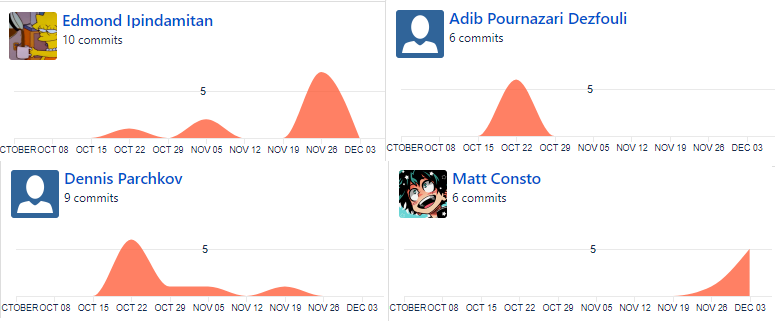
\includegraphics[width=\textwidth]{git}
  \caption{Bitbucket Commit Graphs in the OM2M Repository}
  \label{bitbucket-commit-graphs}
\end{figure}

\begin{figure}[H]
  \centering
  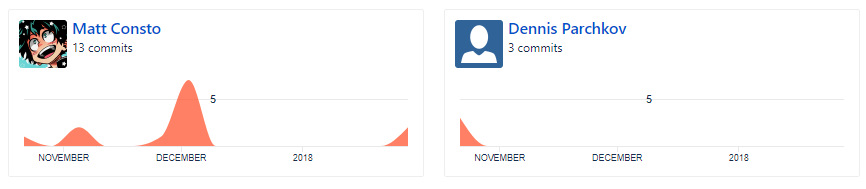
\includegraphics[width=\textwidth]{bitbucket-commit-graphs-2}
  \caption{Bitbucket Commit Graphs in the HATs Repository}
  \label{bitbucket-commit-graphs-2}
\end{figure}

\section{Appendix F - Bitbucket Pipelines}

\begin{figure}[H]
  \centering
  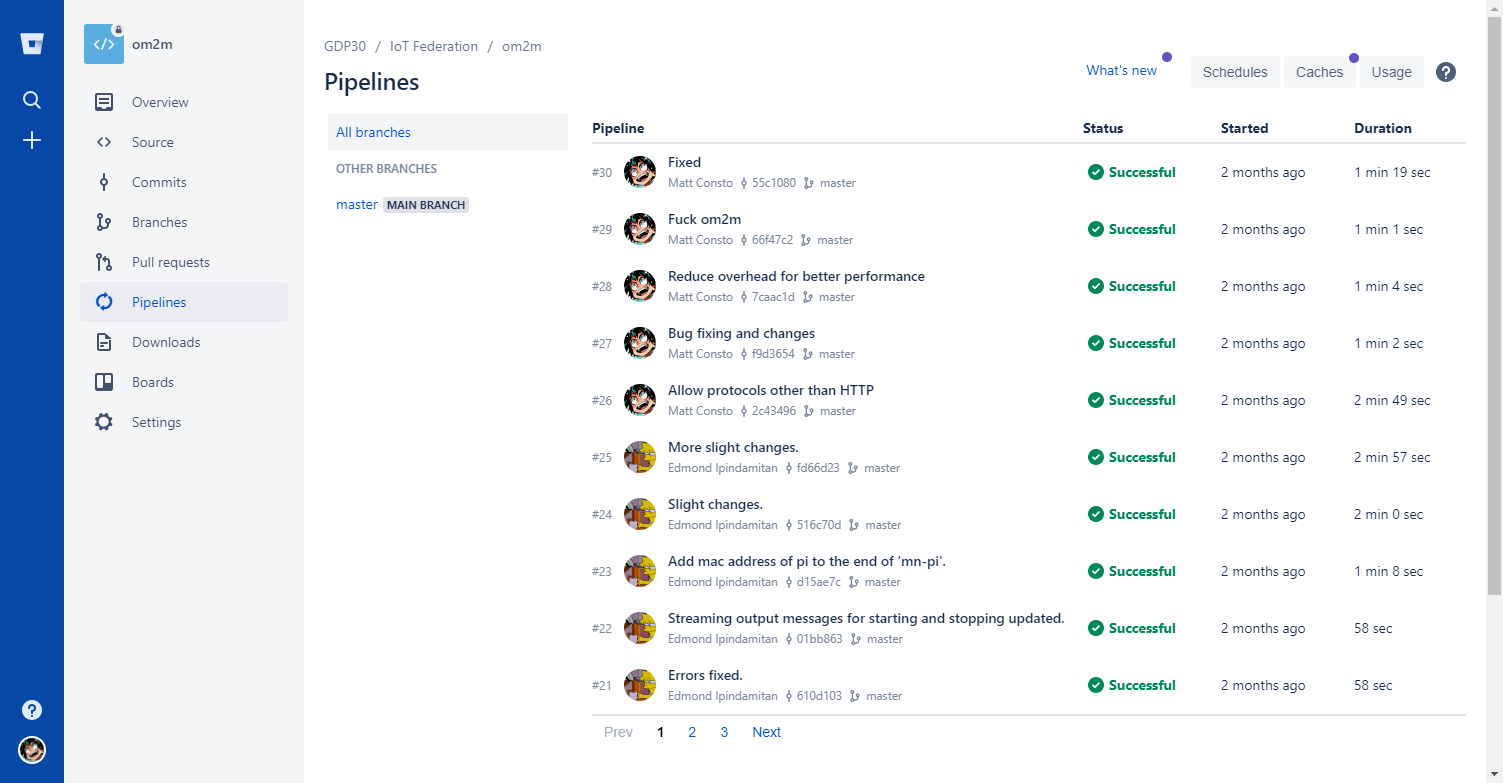
\includegraphics[width=\textwidth]{pipelines}
  \caption{Bitbucket Pipelines}
  \label{bitbucket-pipelines}
\end{figure}

\section{Appendix G - Example of Successful Maven Build \& Install}

\begin{figure}[H]
  \centering
  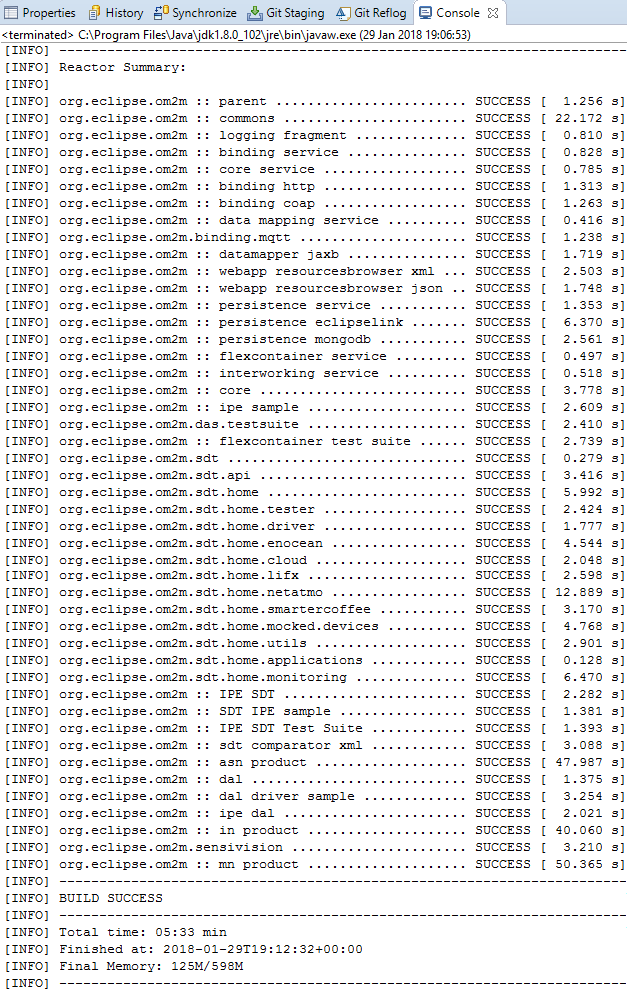
\includegraphics[width=.9\linewidth]{om2mmavensuccess}
  \caption{Maven Build and Install Success}
  \label{maven}
\end{figure}

\section{Appendix H - List of Files in Code Archive}

\dirtree{%
.1 \lstinline{archive.zip}.
.2 \lstinline{readme.md}.
.2 \lstinline{bash}.
.3 \lstinline{gateway.sh}.
.3 \lstinline{sensivision-daemon}.
.3 \lstinline{sensivision-gateway}.
.3 \lstinline{sensivision-server}.
.3 \lstinline{server.sh}.
.2 \lstinline{icons}.
.3 \lstinline{ok.png}.
.3 \lstinline{spinner.png}.
.3 \lstinline{tick.png}.
.3 \lstinline{unknown.png}.
.3 \lstinline{warning_blue.png}.
.3 \lstinline{warning_orange.png}.
.3 \lstinline{warning_red.png}.
.3 \lstinline{warning_yellow.png}.
.3 \lstinline{upscaled}.
.4 \lstinline{ok.png}.
.4 \lstinline{unknown.png}.
.4 \lstinline{warning_red.png}.
.4 \lstinline{warning_yellow.png}.
.2 \lstinline{latex}.
.3 \lstinline{appendices.tex}.
.3 \lstinline{conclusion.tex}.
.3 \lstinline{design.tex}.
.3 \lstinline{ecsgdp.cls}.
.3 \lstinline{evaluation.tex}.
.3 \lstinline{future.tex}.
.3 \lstinline{implementation.tex}.
.3 \lstinline{intro.tex}.
.3 \lstinline{main.tex}.
.3 \lstinline{manual.bib}.
.3 \lstinline{mendeley.bib}.
.3 \lstinline{planning.tex}.
.3 \lstinline{research.tex}.
.3 \lstinline{testing.tex}.
.3 \lstinline{images}.
.4 \lstinline{3ContentInstancesZoom.png}.
.4 \lstinline{bitbucket-commit-graphs-2.png}.
.4 \lstinline{camera.jpg}.
.4 \lstinline{ContentInstance1Zoom.png}.
.4 \lstinline{ContentInstance2Zoom.png}.
.4 \lstinline{ContentInstance3Zoom.png}.
.4 \lstinline{csemodel.png}.
.4 \lstinline{data_storage.PNG}.
.4 \lstinline{errorpicture.jpg}.
.4 \lstinline{fed.png}.
.4 \lstinline{functional.PNG}.
.4 \lstinline{gatt.pdf}.
.4 \lstinline{git.png}.
.4 \lstinline{headers.PNG}.
.4 \lstinline{https.PNG}.
.4 \lstinline{INdata.PNG}.
.4 \lstinline{initial_design.PNG}.
.4 \lstinline{insomnia.PNG}.
.4 \lstinline{lamp.PNG}.
.4 \lstinline{lamps.png}.
.4 \lstinline{nat.PNG}.
.4 \lstinline{nodes.PNG}.
.4 \lstinline{ok.png}.
.4 \lstinline{okpicture.jpg}.
.4 \lstinline{om2minterface2.png}.
.4 \lstinline{om2minterface3.png}.
.4 \lstinline{om2minterface4.PNG}.
.4 \lstinline{om2minterface5.PNG}.
.4 \lstinline{om2mmavensuccess.png}.
.4 \lstinline{om2mpluginstructure.png}.
.4 \lstinline{om2mremotecse.PNG}.
.4 \lstinline{om2m_fed.PNG}.
.4 \lstinline{pi.jpg}.
.4 \lstinline{pipelines.png}.
.4 \lstinline{remotecse.PNG}.
.4 \lstinline{setup.jpg}.
.4 \lstinline{step1.PNG}.
.4 \lstinline{step2.PNG}.
.4 \lstinline{step3.PNG}.
.4 \lstinline{Type2DataZoom.png}.
.4 \lstinline{Type3DataZoom.png}.
.4 \lstinline{Type4DataZoom.png}.
.4 \lstinline{unknown.png}.
.4 \lstinline{unknownpicture.jpg}.
.4 \lstinline{warning_red.png}.
.4 \lstinline{xml.PNG}.
.2 \lstinline{om2m}.
.3 \lstinline{.classpath}.
.3 \lstinline{.gitignore}.
.3 \lstinline{.project}.
.3 \lstinline{build.properties}.
.3 \lstinline{pom.xml}.
.3 \lstinline{META-INF}.
.4 \lstinline{MANIFEST.MF}.
.3 \lstinline{src}.
.4 \lstinline{main}.
.5 \lstinline{java}.
.6 \lstinline{org}.
.7 \lstinline{eclipse}.
.8 \lstinline{om2m}.
.9 \lstinline{sensivision}.
.10 \lstinline{Activator.java}.
.10 \lstinline{RequestSender.java}.
.10 \lstinline{Router.java}.
.10 \lstinline{constants}.
.11 \lstinline{Operations.java}.
.11 \lstinline{SensorConstants.java}.
.10 \lstinline{controller}.
.11 \lstinline{Controller.java}.
.11 \lstinline{LifeCycleManager.java}.
.10 \lstinline{utils}.
.11 \lstinline{ObixUtil.java}.
.11 \lstinline{ProcessManager.java}.
.11 \lstinline{ProcessRunner.java}.
.3 \lstinline{target}.
.4 \lstinline{local-artifacts.properties}.
.4 \lstinline{MANIFEST.MF}.
.4 \lstinline{org.eclipse.om2m.sensivision-1.1.0-SNAPSHOT.jar}.
.4 \lstinline{p2artifacts.xml}.
.4 \lstinline{p2content.xml}.
.4 \lstinline{classes}.
.5 \lstinline{org}.
.6 \lstinline{eclipse}.
.7 \lstinline{om2m}.
.8 \lstinline{sensivision}.
.9 \lstinline{Activator$1$1.class}.
.9 \lstinline{Activator$1.class}.
.9 \lstinline{Activator.class}.
.9 \lstinline{RequestSender.class}.
.9 \lstinline{Router.class}.
.9 \lstinline{constants}.
.10 \lstinline{Operations.class}.
.10 \lstinline{SensorConstants.class}.
.9 \lstinline{controller}.
.10 \lstinline{Controller.class}.
.10 \lstinline{LifeCycleManager.class}.
.9 \lstinline{utils}.
.10 \lstinline{ObixUtil.class}.
.10 \lstinline{ProcessManager.class}.
.10 \lstinline{ProcessRunner.class}.
.4 \lstinline{generated-sources}.
.5 \lstinline{annotations}.
.4 \lstinline{maven-archiver}.
.5 \lstinline{pom.properties}.
.2 \lstinline{openmtc}.
.3 \lstinline{start.py}.
.2 \lstinline{python}.
.3 \lstinline{accelerometer.py}.
.3 \lstinline{blink.py}.
.3 \lstinline{clear.py}.
.3 \lstinline{compass.py}.
.3 \lstinline{cpu.py}.
.3 \lstinline{disk.py}.
.3 \lstinline{gyroscope.py}.
.3 \lstinline{humidity.py}.
.3 \lstinline{joystick.py}.
.3 \lstinline{lowlight.py}.
.3 \lstinline{memory.py}.
.3 \lstinline{orientation.py}.
.3 \lstinline{pixels.py}.
.3 \lstinline{pressure.py}.
.3 \lstinline{process.py}.
.3 \lstinline{quality.py}.
.3 \lstinline{rotation.py}.
.3 \lstinline{scroll.py}.
.3 \lstinline{temperature.py}.
.3 \lstinline{time.py}.
.3 \lstinline{wifi.py}.
.2 \lstinline{tests}.
.3 \lstinline{integration.py}.
.3 \lstinline{test.py}.
.2 \lstinline{video}.
.3 \lstinline{fetch.php}.
.3 \lstinline{index.html}.
}

\clearpage
